\documentclass[frenchb, oneside, headings=normal]{scrartcl}

\usepackage[utf8x]{inputenc}
\usepackage[T1]{fontenc}
\usepackage{lmodern}

\usepackage{ifthen}
\usepackage{url}


\usepackage{multirow}

% Color
% cfr http://en.wikibooks.org/wiki/LaTeX/Colors
\usepackage{color}
\usepackage[usenames,dvipsnames,svgnames,table]{xcolor}
\definecolor{dkgreen}{rgb}{0.25,0.7,0.35}
\definecolor{dkred}{rgb}{0.7,0,0}

\newcommand{\matlab}{\textsc{Matlab}}

% Math symbols
\usepackage{amsmath}
\usepackage{amssymb}
\usepackage{amsthm}
\DeclareMathOperator*{\argmin}{arg\,min}
\DeclareMathOperator*{\argmax}{arg\,max}


% Sets
\newcommand{\Z}{\mathbb{Z}}
\newcommand{\R}{\mathbb{R}}
\newcommand{\Rn}{\R^n}
\newcommand{\Rnn}{\R^{n \times n}}
\newcommand{\C}{\mathbb{C}}
\newcommand{\K}{\mathbb{K}}
\newcommand{\Kn}{\K^n}
\newcommand{\Knn}{\K^{n \times n}}

% Unit vectors
\usepackage{esint}
\usepackage{esvect}
\newcommand{\kmath}{k}
\newcommand{\xunit}{\hat{\imath}}
\newcommand{\yunit}{\hat{\jmath}}
\newcommand{\zunit}{\hat{\kmath}}
\newcommand{\uunit}{\hat{\umath}}

% rot & div & grad & lap
\DeclareMathOperator{\newdiv}{div}
\newcommand{\divn}[1]{\nabla \cdot #1}
\newcommand{\rotn}[1]{\nabla \times #1}
\newcommand{\grad}[1]{\nabla #1}
\newcommand{\gradn}[1]{\nabla #1}
\newcommand{\lap}[1]{\nabla^2 #1}


% Elec
\newcommand{\B}{\vec B}
\newcommand{\E}{\vec E}
\newcommand{\EMF}{\mathcal{E}}
\newcommand{\perm}{\varepsilon} % permittivity

\newcommand{\bigoh}{\mathcal{O}}
\newcommand\eqdef{\triangleq}

\DeclareMathOperator{\newdiff}{d} % use \dif instead
\newcommand{\dif}{\newdiff\!}
\newcommand{\fpart}[2]{\frac{\partial #1}{\partial #2}}
\newcommand{\ffpart}[2]{\frac{\partial^2 #1}{\partial #2^2}}
\newcommand{\fdpart}[3]{\frac{\partial^2 #1}{\partial #2\partial #3}}
\newcommand{\fdif}[2]{\frac{\dif #1}{\dif #2}}
\newcommand{\ffdif}[2]{\frac{\dif^2 #1}{\dif #2^2}}
\newcommand{\constant}{\ensuremath{\mathrm{cst}}}

\usepackage{siunitx}

\usepackage{tikz}

\usepackage{pgfplots}
\usepackage{lmodern}
\usepackage{microtype}
\usepackage{xspace}

\usepackage{babel}
% Listing
% always put it after babel
% http://tex.stackexchange.com/questions/100717/code-in-lstlisting-breaks-document-compile-error
\usepackage{listings}

\definecolor{mygreen}{rgb}{0,0.6,0}
\definecolor{mygray}{rgb}{0.5,0.5,0.5}
\definecolor{mymauve}{rgb}{0.58,0,0.82}
\lstset{ %
  language=Matlab,
  backgroundcolor=\color{white},   % choose the background color; you must add \usepackage{color} or \usepackage{xcolor}
  basicstyle=\footnotesize,        % the size of the fonts that are used for the code
  breakatwhitespace=false,         % sets if automatic breaks should only happen at whitespace
  breaklines=true,                 % sets automatic line breaking
  captionpos=b,                    % sets the caption-position to bottom
  commentstyle=\color{mygreen},    % comment style
  deletekeywords={...},            % if you want to delete keywords from the given language
  escapeinside={\%*}{*)},          % if you want to add LaTeX within your code
  extendedchars=true,              % lets you use non-ASCII characters; for 8-bits encodings only, does not work with UTF-8
  frame=single,	                   % adds a frame around the code
  keepspaces=true,                 % keeps spaces in text, useful for keeping indentation of code (possibly needs columns=flexible)
  keywordstyle=\color{blue},       % keyword style
  otherkeywords={*,...},           % if you want to add more keywords to the set
  numbers=none,                    % where to put the line-numbers; possible values are (none, left, right)
  numbersep=5pt,                   % how far the line-numbers are from the code
  numberstyle=\tiny\color{mygray}, % the style that is used for the line-numbers
  rulecolor=\color{black},         % if not set, the frame-color may be changed on line-breaks within not-black text (e.g. comments (green here))
  showspaces=false,                % show spaces everywhere adding particular underscores; it overrides 'showstringspaces'
  showstringspaces=false,          % underline spaces within strings only
  showtabs=false,                  % show tabs within strings adding particular underscores
  stepnumber=2,                    % the step between two line-numbers. If it's 1, each line will be numbered
  stringstyle=\color{mymauve},     % string literal style
  tabsize=2,	                   % sets default tabsize to 2 spaces
  title=\lstname                   % show the filename of files included with \lstinputlisting; also try caption instead of title
}

\KOMAoptions{DIV=last}

\usepackage[top = 2.5 cm, bottom = 3 cm, left = 2.5 cm, right = 2.5 cm]{geometry}
\usepackage{caption}


\usepackage{epstopdf}
\usepackage{wrapfig}
\usepackage{verbatim}
\begin{document}

\title{Projet ELEC Master 1 - Labo 5}
\subtitle{Groupe 4}
\author{Deprez Damien \and Bilal Ouachalih }
\date{18 november 2016}
\maketitle

The purpose of this lab is to correct the frequency offset and the delay due to the channel.

\section{Questions of the Pre-Lab}

\subsection{Describe what happens to the error rate of your system when the estimate for the delay in the channel is off by more than one symbol time}

First, we modified a little bit the schematic of the SlidingCorrelation.vi. In fact, we have added a controller to make an error on the delay to let us observe what happen. Here is the result\\

\begin{center}
	\begin{tabular}{c|c|c}
		 Equalizer Length & Correct delay + error & BER\\
		\hline
		 4& 3 & 0.074\\
		  & 4 & 0.5 \\
		  \hline
		 5 & 4  & 0  \\
		   & 5  & 0.488  \\
		  \hline
		6 & 5  & 0 \\
		 &  6  & 0.504 \\   
	\end{tabular}
	\captionof{table}{Effect of the error introduced in the delay on the BER}
	\label{BER_equ_length_4}
    \end{center}

\begin{comment}
\begin{figure}[!ht]
  \begin{minipage}[b]{0.48\linewidth}
        \centering 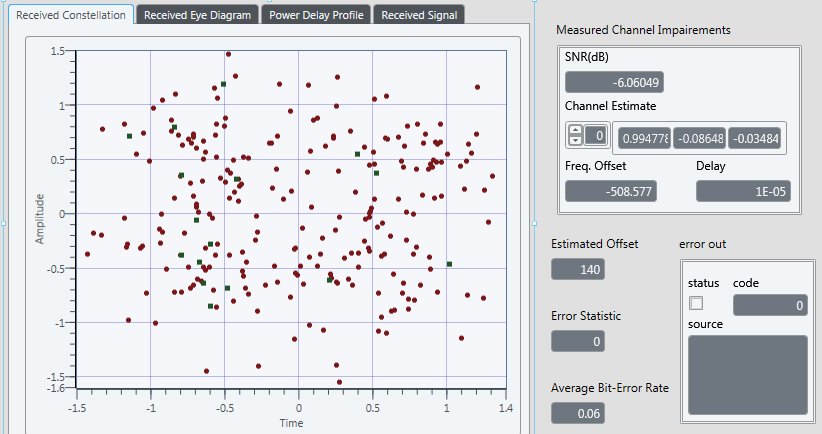
\includegraphics[scale=0.45]{img/Sliding_correletaion_OFF_AWGN_5dB_shift_bit_0.png}
    \caption{Error rate for a delay+0 in AWGN}
    \label{fig1}
    \end{minipage}\hfill
    \begin{minipage}[b]{0.48\linewidth}
         \centering 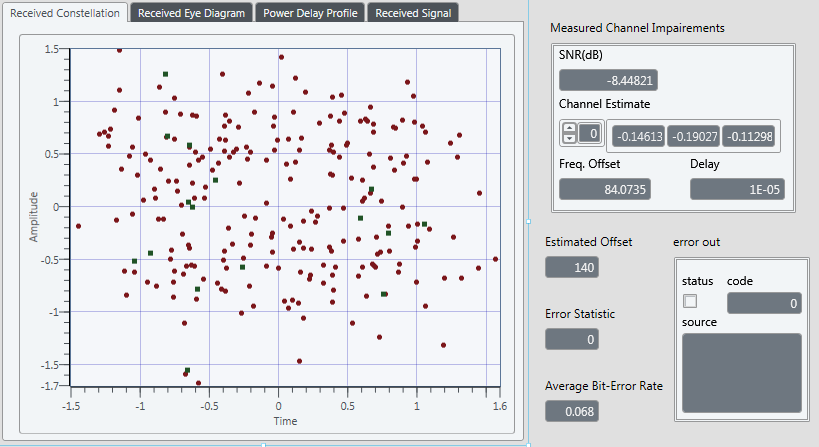
\includegraphics[scale=0.45]{img/Sliding_correletaion_OFF_AWGN_5dB_shift_bit_1.png}
          \caption{Error rate for a delay+1 in AWGN}
          \label{fig2}
    \end{minipage}
\end{figure}

\begin{figure}[!ht]
    \begin{minipage}[b]{0.48\linewidth}
        \centering 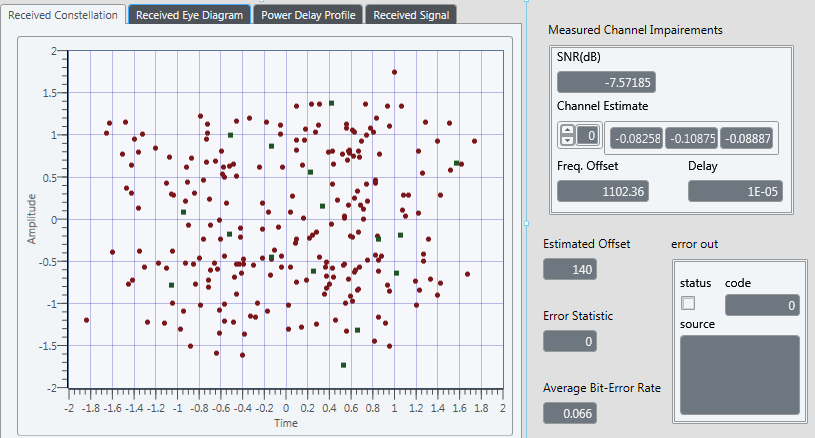
\includegraphics[scale=0.45]{img/Sliding_correletaion_OFF_AWGN_5dB_shift_bit_2.png}
     \caption{Error rate for a delay+2 in AWGN}
     \label{fig3}
    \end{minipage}\hfill
    \begin{minipage}[b]{0.48\linewidth}
         \centering 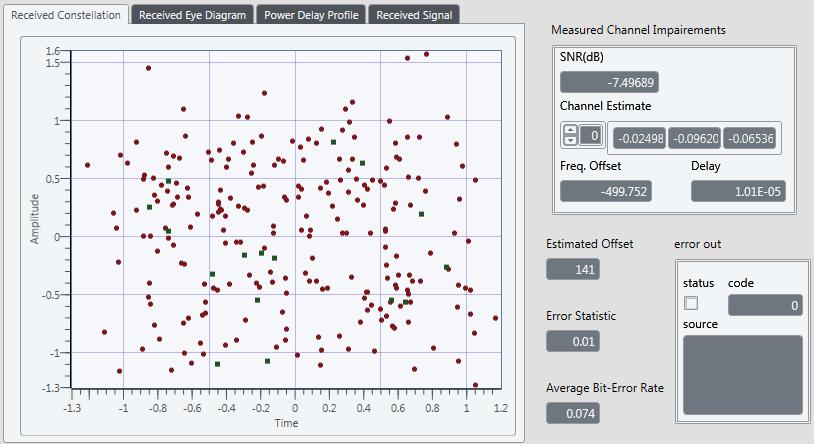
\includegraphics[scale=0.45]{img/Sliding_correletaion_OFF_AWGN_5dB_shift_bit_3.PNG}
          \caption{Error rate for a delay+3 in AWGN}
          \label{fig4}
    \end{minipage}  

\end{figure}
\begin{figure}[!ht]
    \begin{minipage}[b]{0.48\linewidth}
        \centering 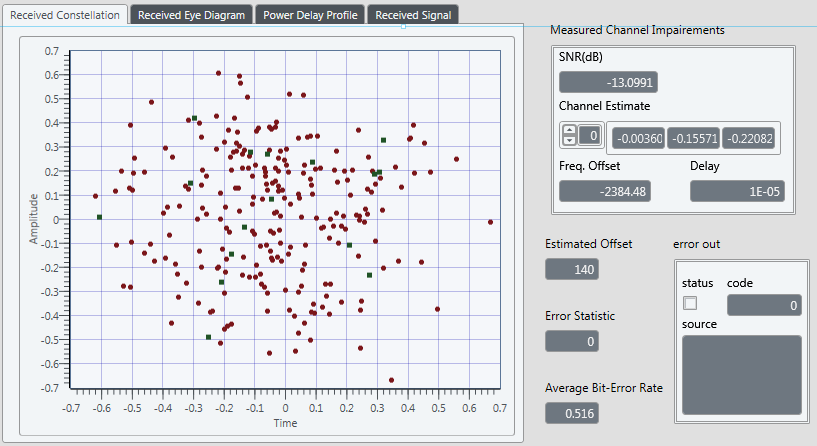
\includegraphics[scale=0.45]{img/Sliding_correletaion_OFF_AWGN_5dB_shift_bit_4.PNG}
     \caption{Error rate for a delay+4 in AWGN}
     \label{fig5}
    \end{minipage}\hfill
    \begin{minipage}[b]{0.48\linewidth}
         \centering 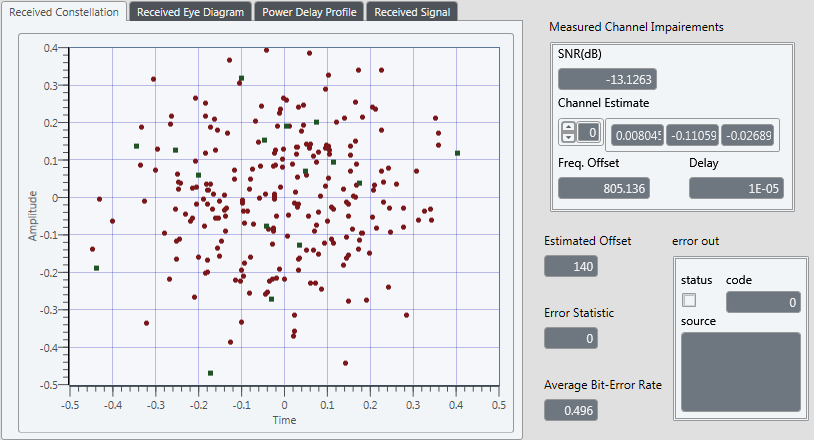
\includegraphics[scale=0.45]{img/Sliding_correletaion_OFF_AWGN_5dB_shift_bit_5.PNG}
 \caption{Error rate for a delay+5 in AWGN}\label{fig6}
    \end{minipage}
\end{figure}
\end{comment}

As we can in the table \ref{BER_equ_length_4}, that when the delay plus the error we intentionally add equal $L-1$, with L the length of the equalizer, we have a BER of $\simeq 0.5$. Which means that one symbol on two is not well placed. Here is an illustration of that phenomena.

\begin{figure}[!ht]
    \begin{minipage}[b]{0.48\linewidth}
        \centering 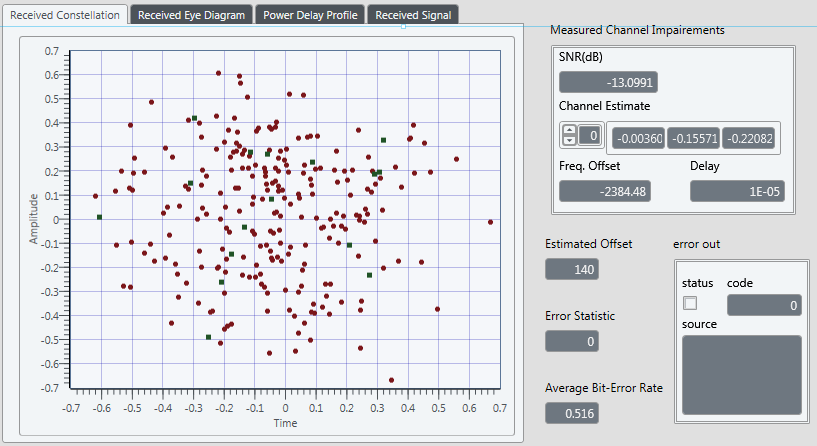
\includegraphics[scale=0.45]{img/Sliding_correletaion_OFF_AWGN_5dB_shift_bit_4.PNG}
     \caption{Error rate for a delay+4 in AWGN}
     \label{fig5}
    \end{minipage}\hfill
    \begin{minipage}[b]{0.48\linewidth}
         \centering 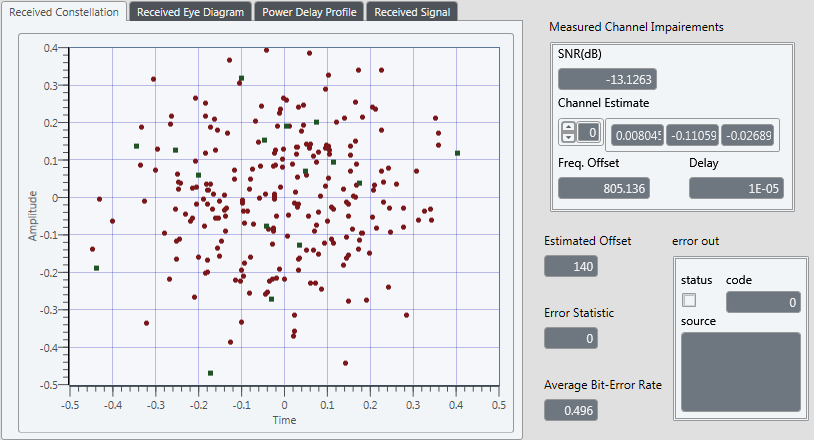
\includegraphics[scale=0.45]{img/Sliding_correletaion_OFF_AWGN_5dB_shift_bit_5.PNG}
 \caption{Error rate for a delay+5 in AWGN}\label{fig6}
    \end{minipage}
\end{figure}

%%As we can seen on figure \ref{fig1},\ref{fig2},\ref{fig3} and \ref{fig4}, we have the error rate which is yet acceptable for an added delay of 0 to 3. But on figure \ref{fig5} and \ref{fig6}, when we add to the estimated delay, 4, we have a bit error rate of $\simeq 0.5$, which is very bad. Which means that one bit on two is not well placed. 

\subsection{Describe what happens to the received constellation if you do not correct for the 201 Hz frequency offset}

When we set the controller of the frequency offset on FALSE, we don't correct the error of frequency anymore, and we obtain the following result

\begin{figure}[!ht]
\centering
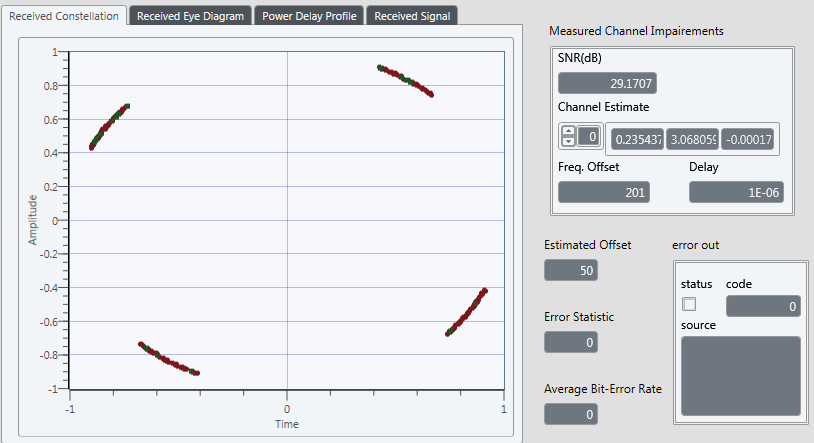
\includegraphics[scale=0.7]{img/test_offset_201hz_OFF.PNG}
\caption{Constellation for a frequency offset of $201 \si{\hertz}$ without correction}
\label{freq_correct_off}
\end{figure}

On the figure \ref{freq_correct_off}, we can see  that we don't have a nice constellation with 4 clear points in the 4 corner, but multiple points distributed on a portion of circle.

\subsection{What are the range of frequency offsets that you can estimate/correct using the Moose algorithm?}

If we based our observation on what is said in the book, we can determine the range of frequency to have a good work of the Moose method. In fact, we have this condition

\begin{equation}
|\epsilon| \leq \frac{1}{2*N_t} = \frac{1}{2*44} = 0.01136
\label{cdt1}
\end{equation}

Or in an other form 

\begin{equation}
|f_e| \leq \frac{1}{2*T*N_t} = \frac{1}{2*1e-6*44} \simeq 11 \si{\kilo\hertz}
\label{cdt2}
\end{equation}\\

So, if we have a frequency offset greater then $11 \si{\kilo\hertz}$, the Moose method will not work anymore. In order to check if we are right, we made two simulations. The first one with a frequency offset of $10 \si{\kilo\hertz}$ and an other with $12 \si{\kilo\hertz}$, and the result is interesting.\\

\begin{figure}[!ht]
    \begin{minipage}[b]{0.48\linewidth}
        \centering 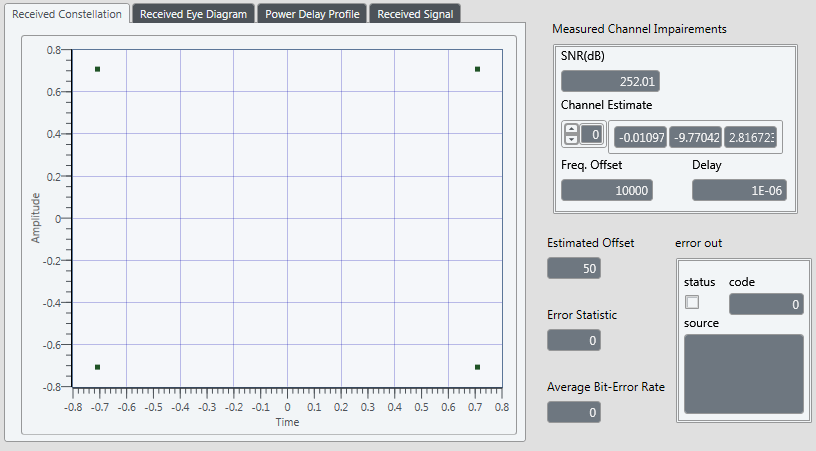
\includegraphics[scale=0.45]{img/test_Offset_10k_OK_limitMooseCheck.png}
     \caption{Simulation with a frequency offset of $10 \si{\kilo\hertz}$}
     \label{MooseLimit1}
    \end{minipage}\hfill
    \begin{minipage}[b]{0.48\linewidth}
         \centering 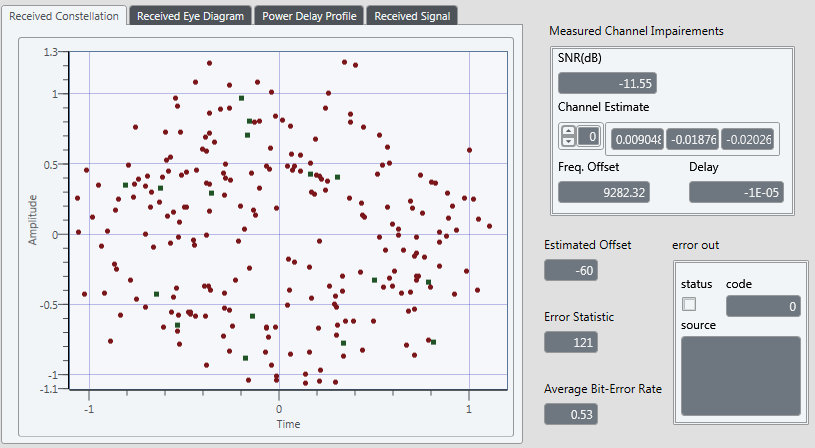
\includegraphics[scale=0.45]{img/test_Offset_12k_OK_limitMooseCheck.png}
\caption{Simulation with a frequency offset of $12 \si{\kilo\hertz}$}
 \label{MooseLimit2}
    \end{minipage}
\end{figure}

On the figure \ref{MooseLimit1} and \ref{MooseLimit2}, the result speaks of himself. Moose method doesn't work anymore above $\simeq 11 \si{\kilo\hertz}$.

\section{Question of the Lab}

\subsection{Before changing any of the settings, calculate an average value (using five runs or so) of the inherent offset between the transmitter and receiver.}

We run five times the receiver program and we obtain the following result
 
\begin{center}
	\begin{tabular}{c|c}
		run & frequency offset [\si{\hertz}]\\
		\hline
		1 & 7.75\\
		2 & 12.74\\
		3 & 5.73\\
		4 & -5.26\\
		5 & -1.158\\
	\end{tabular}
\end{center}

The average offset between the transmitter and receiver is $3.96$ \si{\hertz}. 


\subsection{Based on the system parameters, what is the range of frequency offsets that can be estimated by your frequency offset estimation algorithm?}

Like in the previous section, we use the equation \ref{cdt1} and \ref{cdt2}, to determine the range of frequency. In the case of USRP transmission, the range of admissible frequency offset is between $0$ and $2272 \si{\hertz}$.

\subsection{Let fM be the maximum correctable frequency offset of your system (i.e., as calculated in the previous question). Modify the carrier frequency of your transmitter so that you will cause an effective offset of 0.80fM at the receiver. What is the new value of the carrier frequency at your transmitter?}

If we make a test with the USRP, and we add to the carrier frequency $0.8*f_m=0.8*2272=1818 \si{\hertz}$, we obtained the following result

\begin{figure}[!ht]
  \begin{minipage}[b]{0.48\linewidth}
        \centering 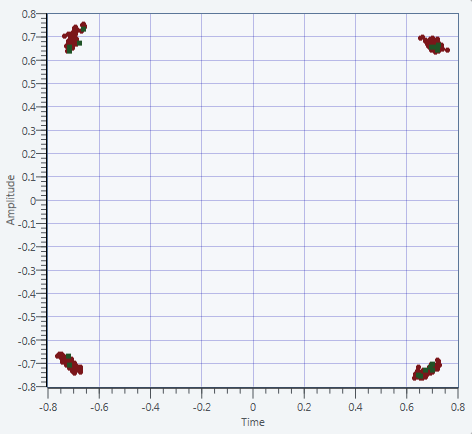
\includegraphics[scale=0.7]{img/USRP_carrieroffset_227.PNG}
    \caption{Result for a frequency offset of $227 \si{\hertz}$}
    \label{fig8}
    \end{minipage}\hfill
    \begin{minipage}[b]{0.48\linewidth}
         \centering 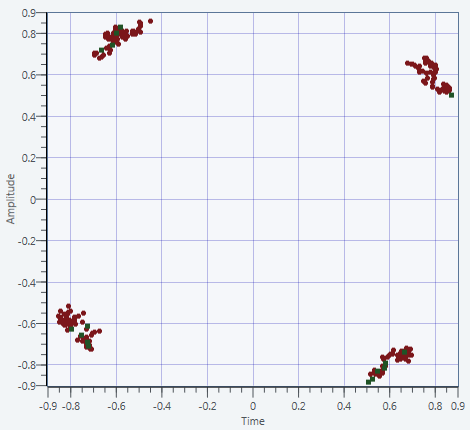
\includegraphics[scale=0.7]{img/USRP_carrieroffset_1818.PNG}
          \caption{Result for a frequency offset of $1818 \si{\hertz}$}
          \label{fig9}
    \end{minipage}
\end{figure}

On figures \ref{fig8} and \ref{fig9}, We can observe that, more we increase the frequency offset near the maximum one, more the point on the constellation are not perfectly centered in the 4 corner of the figure.

\begin{figure}[!ht]
    \begin{minipage}[b]{0.48\linewidth}
        \centering 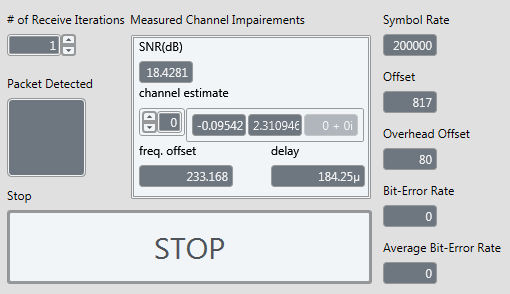
\includegraphics[scale=0.7]{img/USRP_value_227.PNG}
     \caption{Result data for a frequency offset of $227 \si{\hertz}$}
     \label{fig10}
    \end{minipage}\hfill
    \begin{minipage}[b]{0.48\linewidth}
         \centering 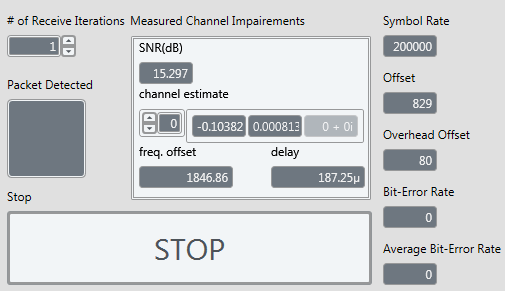
\includegraphics[scale=0.7]{img/USRP_value_1818.PNG}
          \caption{Result data for a frequency offset of $1818 \si{\hertz}$}
          \label{fig11}
    \end{minipage}  
\end{figure}

The figures \ref{fig10} and \ref{fig11} show the result given by the topRX.vi, and show that, the frequency offset inserted at the transmitter is very similar to the one he measure at the receiver. Which means, that the channel itself doesn't introduce a significative error in frequency, but more in the delay.
\newpage
\section{Self referenced frame synchronization}

We are going to explore another algorithm more robust to frequency offset. In fact, the presented before, like said in previous question, "break" under large frequency offset.

First, let's consider the following received sequence

\begin{equation}
y[n] = 	\alpha \exp^{j2\pi \epsilon n}t[n-D]
\label{equ} 
\end{equation}

where $t[n]$ is the transmitted sequence, $\alpha$ is a complex scalar and D is the delay 	introduced by the channel.

\subsection{Why the self referenced frame detector works better than the correlation based detector under large frequency offsets.}

If we study the following equation

\begin{equation}
\hat{d}=argmax \frac{\sum_{n=L}^{N_t-1} y(n+d+N_t)+y(n+d)^*}{\sqrt{\sum_{n=L}^{N_t-1} |y(n+d)|^2}\sqrt{\sum_{n=L}^{N_t-1} |y(n+d+N_t)|^2}}
\end{equation}\\

We can see that, if we develop the numerator, we can prove that it is independant of $\epsilon$ (the frequency offset). In fact, by the expression \ref{equ}, we have

\begin{equation}
y[n+d]^*= \alpha \exp^{-j2\pi \epsilon (n+d)}t[n+d-D]^*
\end{equation}
\begin{equation}
y[n+d+N_t]= \alpha \exp^{j2\pi \epsilon (n+d+N_t)}t[n+d+N_t-D]
\end{equation}
\begin{equation}
|y[n+d+N_t]*y[n+d]^*| = \alpha^2*|t[n+d-D]t[n+d+N_t-D]|
\label{equ2}
\end{equation} 	

We take the module of $y[n+d+N_t]*y[n+d]^*$ because y can be complex. And in the equation \ref{equ2}, we have no more $\epsilon$ appearing.
At the end, we can conclude that, for this method, the estimation of the delay will not depend of the frequency offset. 

\subsection{Name three impairments in a real wireless system which impact the accuracy of the correlation based detection method.}

The 3 impairements are\\ 

\begin{itemize}

\item \textbf{The frequency offset}, if we have a frequency offset, the correlation of the received training sequence will be less effective.

\item \textbf{the noise} can make the calcul of the correlation difficult because, we will receive a sequence corrupted by noise.

\item \textbf{the intersymbol interference}, if we have some symbols shifted and near another, the correllation will be less effective.
\end{itemize}

\subsection{Under large frequency offsets, the correlation based detector “breaks”. What property of the training sequence breaks down under large frequency offsets?}

We know that the training sequence has a very good correlation. But, with the correlation based detector, the Moose algorithm has a maximum admissible frequency offset. If the offset become too large, the property of good correlation of the training sequence will be no more fulfilled. In fact, in case of too large offset, the symbol will be too far away, and the correlation with the training sequence will have no more sense.

\subsection{In the self referenced frame synchronization method, is it still critical that the periodic training sequence have good autocorrelation properties? If so, why?}

I think we can't say that it's no more critical that the periodic training sequence must still have good autocorrelation properties. In faimit frequency of the Moose algorithm. When we try the new algorithm with larger offset, we can see that there is still a limit to the span of frequency we can consider. But, the range is larger then with the former method. In fact,we have bad result around $22.5$ \si{\kilo\hertz}.

\begin{figure}[!ht]
    \begin{minipage}[b]{0.48\linewidth}
        \centering 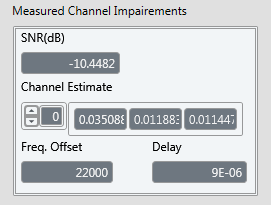
\includegraphics[scale=0.65]{img/NewMethodLimit_22k.PNG}
     \caption{Measured data for a frequency offset of $22 \si{\kilo\hertz}$}
     \label{fig10}
    \end{minipage}\hfill
    \begin{minipage}[b]{0.48\linewidth}
         \centering 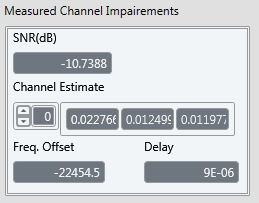
\includegraphics[scale=0.7]{img/NewMethodLimit_23k}
          \caption{Mesured data for a frequency offset of $23 \si{\kilo\hertz}$}
          \label{fig11}
    \end{minipage}  
\end{figure}

\end{document}
